\documentclass[12pt]{article}
\usepackage[top=3cm, left=3cm, right=3cm]{geometry}
\usepackage[utf8]{inputenc}
\usepackage[english]{babel}
\usepackage{times}
\usepackage{calc}
\usepackage{eso-pic}
\usepackage{titlesec}
\usepackage{array}
\usepackage{makecell}
\usepackage{graphicx}
\usepackage{tikz-uml}
\usepackage{pgfgantt}

% \date{06 Oct, 2024}
\title{Cloud Maker}
\author{Vikas Kushwaha}

\nonstopmode

\newlength{\PageFrameTopMargin}
\newlength{\PageFrameBottomMargin}
\newlength{\PageFrameLeftMargin}
\newlength{\PageFrameRightMargin}

\setlength{\PageFrameTopMargin}{1cm}
\setlength{\PageFrameBottomMargin}{1cm}
\setlength{\PageFrameLeftMargin}{1cm}
\setlength{\PageFrameRightMargin}{1cm}

\makeatletter

\let\inserttitle\@title
\let\insertauthor\@author
\let\insertdate\@date

\newlength{\Page@FrameHeight}
\newlength{\Page@FrameWidth}

\AddToShipoutPicture {
	\thicklines
	\setlength{\Page@FrameHeight}{\paperheight-\PageFrameTopMargin-\PageFrameBottomMargin}
	\setlength{\Page@FrameWidth}{\paperwidth-\PageFrameLeftMargin-\PageFrameRightMargin}
	\put(\strip@pt\PageFrameLeftMargin,\strip@pt\PageFrameTopMargin){
		\framebox(\strip@pt\Page@FrameWidth, \strip@pt\Page@FrameHeight){}}}

\makeatother

\titleformat{\section}
{\Large\bfseries\center\uppercase}
{}
{1em}
{}
[\hrule]

\AddToHook{cmd/section/before}{\clearpage}
% \tikzumlset{fill usecase=white}
\graphicspath{ {./images/} }

\newenvironment{changemargin}[2]{%
\begin{list}{}{%
\setlength{\topsep}{0pt}%
\setlength{\leftmargin}{#1}%
\setlength{\rightmargin}{#2}%
\setlength{\listparindent}{\parindent}%
\setlength{\itemindent}{\parindent}%
\setlength{\parsep}{\parskip}%
}%
\item[]}{\end{list}}

\renewcommand\theadfont{\bfseries}


\begin{document}

\begin{center}
	\fontsize{14pt}{28pt}\selectfont
	A PROJECT REPORT \\
	on \\
	\textbf{"\underline{\MakeUppercase{\inserttitle}}"} \\
	\textit{submitted by} \\
	\textbf{Mr. \insertauthor} \\
	\textbf{Seat No :-} \\
	\textit{in partial fullfillment for the award of the degree} \\
	of \\
	\textbf{BACHELOR OF SCIENCE} \\
	in \\
	\textbf{COMPUTER SCIENCE} \\
	\textit{under the guidance of} \\
	\textbf{Mrs. Swetha Iyer} \\
	\textbf{Department of Computer Science} \\
	\bigskip
\includegraphics[scale=0.25]{vartak-logo} \\
	\fontsize{14pt}{20pt}\selectfont
	\textbf{VIDYAVARDHINI'S} \\
	\textbf{A. V. COLLEGE OF ARTS, K. M. COLLEGE OF COMMERCE} \\
	\textbf{E. S. A. COLLEGE OF SCIENCE,} \\
	\textbf{VASAI(WEST), PALGHAR-401208, MAHARASHTRA} \\
	\textbf{(Sem V)} \\
	\fontsize{14pt}{28pt}\selectfont
	\textbf{(2024-25)} \\
\end{center}


\fontsize{12pt}{24pt}\selectfont

\section{Acknowledgement}
\begin{center}
	\vspace{2cm}
	I would like to acknowledge my sincere thanks towards our project guide \\
	\textbf{Head of Computer Scince Department} \\
	\textbf{Mrs. Srimathi Narayanan} \\
	for their valuable guidance and suggestions and \\
	providing me an opportunity to do the project work in the college lab and \\
	which made me complete the project successfully. \\
	\vspace{2cm}
	I am also thankful to \\
	\textbf{Mrs. Gyaneshwari Pawar} \\
	For providing such nice guidance in form of comments and corrections. \\
	I am thakful to and fortunate enough to get contant encouragement, \\
	support and guidance from all teaching staff of Computer Science \\
	which helped us in successfully completing our project work. \\
Also, I would like to extend our sincere esteems to all staff in laboratory \\
	for their timely support. \\
	\vspace{2cm}
	By \textbf{\insertauthor}, \\
	T.Y.BSc (Computer Science)
\end{center}


\section{Declaration}
\vspace{2cm}
I \textbf{\underline{\insertauthor}} hereby declare that, \\
\bigskip \\
The project entitled
\textbf{"\underline{\MakeUppercase{\inserttitle}}"}
submitted in the partial fulfillment for the award of Bachelor of Science in Computer Science during the academic year \textbf{2023 - 2024} is my original work and the project has not formed the basis for the award of any degree, associate ship, fellowhip or any other similar titles. \\ \\ \\
\vspace{2cm}
\textbf{Signature of the Student:} \\
\bigskip
\textbf{Place:} \\
\bigskip
\textbf{Date:} \\

\fontsize{12pt}{18pt}\selectfont

\section{Event Table}
\begin{changemargin}{-1cm}{-1cm}
\vfill
\begin{center}
\begin{tabular}{ | m{2cm} | m{3.5cm} | m{1.5cm} | m{4cm} | m{2cm} | m{2cm} | }
	\hline
	\thead{Event} &
	\thead{Trigger} &
	\thead{Source} &
	\thead{Activity} &
	\thead{Response} &
	\thead{Destination} \\
	\hline\hline
	Cut Files &
	User clicks on Cut Button & User &
	Files are added to Cut Buffer &
	Files in Cut Buffer &
	Endpoint Server \\ \hline

	Copy Files & User clicks on Copy Button & User &
	Files are added to Copy Buffer &
	Files in Copy Buffer &
	Endpoint Server \\ \hline

	Paste from Cut Buffer &
	User clicks on Paste button &
	User &
	Files are moved from Cut Buffer &
	Files Moved &
	Endpoint Server \\ \hline

	Paste from Copy Buffer &
	User clicks on Paste button &
	User &
	Files are copied from Copy Buffer &
	Files Copied &
	Endpoint Server \\ \hline

	Delete Files &
	User clicks on Delete Button &
	User &
	Selected Files are set to deletion &
	Confirm Deletion &
	Endpoint Server \\ \hline

	Upload Local Files &
	User clicks on Upload Button &
	User &
	File Browser is opened for selection &
	User submits files &
	User \\ \hline

	Download Remote Files &
	Server gets Download Requests &
	Endpoint Server &
	Server ZIPs requested file and sends to user &
	Compressed File recieved &
	User \\ \hline

	Create Folder &
	User enters New Folder Name &
	User &
	New Folder is created on the system &
	Folder is shown &
	Endpoint Server \\ \hline

\end{tabular}
\end{center}
\vfill
\end{changemargin}


\section{Class Diagram}
\vfill
\begin{center}
\begin{tikzpicture}[
		class/.style={minimum width=6cm},
	]
	\umlclass[class]{FSData}{
		CutCount: int \\
		CopyCount: int \\
		FileCount: int \\
		CutBuffer: []string \\
		CopyBuffer: []string \\
		File: *FileNode \\
	}{}
	\umlclass[class, x=8cm, y=-8cm]{FileNode}{
		URI: string \\
		Path: string \\
		IsDir: bool \\
		Info: os.FileInfo \\
		Data: any \\
	}{
		HTMLPath(): template.HTML \\
		EvalSymlinks(): string \\
		IconPath(): string \\
		Size(): string \\
		Mode(): string \\
		ModDate(): string \\
		ModTime(): string \\
		Details(): string \\
	}
	\umluniaggreg[geometry=-|]{FSData}{FileNode}
\end{tikzpicture}
\end{center}
\vfill


% \section{ER Diagram}
% \vfill
% \begin{center}
% \begin{tikzpicture}[
% 		class/.style={minimum width=4cm},
% 	]
% 	\umlclass[class]{FSData}{
% 		CutCount \\
% 		CopyCount \\
% 		FileCount \\
% 		CutBuffer \\
% 		CopyBuffer \\
% 		File \\
% 	}{}
% 	\umlclass[class, x=8cm, y=-8cm]{FileNode}{
% 		URI \\
% 		Path \\
% 		IsDir \\
% 		Info \\
% 		Data \\
% 	}{}
% 	\umlassoc[geometry=-|]{FSData}{FileNode}
% \end{tikzpicture}
% \end{center}
% \vfill


\section{Use Case Diagram}
\vfill
\begin{center}
\begin{tikzpicture}[
		case/.style={text width=3cm},
		subcase/.style={minimum width=3cm}
	]
	\begin{umlsystem}[x=6] {}
		\umlusecase[case, name=br] {Browse Files Remotely}
		\umlusecase[case, name=ob, x=6cm, y=-2cm] {Open in Browser}
		\umlusecase[case, name=up, y=-3cm] {Upload Files}
		\umlusecase[case, name=dn, y=-5cm] {Download Files}
		\umlusecase[case, name=fm, y=-8cm] {Manage Files}
		\umlusecase[subcase, name=cp, x=6cm, y=-6cm] {Copy}
		\umlusecase[subcase, name=mv, x=7cm, y=-8cm] {Move}
		\umlusecase[subcase, name=dl, x=6cm, y=-10cm] {Delete}
	\end{umlsystem}
	\node [above] at (current bounding box.north) {Cloud Maker};
	\umlactor[y=-4] {User}
	\umlassoc{User}{br}
	\umlassoc{User}{up}
	\umlassoc{User}{dn}
	\umlassoc{User}{fm}
	\umlextend{br}{ob}
	\umlinclude{fm}{cp}
	\umlinclude{fm}{mv}
	\umlinclude{fm}{dl}
\end{tikzpicture}
\end{center}
\vfill


\section{Sequence Diagram}
\vfill
Stage 1: Connect to Cloud Storage \\
\begin{center}
\begin{tikzpicture}
\begin{umlseqdiag}
	\umlactor[class=User]{u}
	\umlobject[x=7, class=Server]{proxy}
	\umlobject[x=14, class=Server]{endpoint}

	\begin{umlcall}[op=Port Forwarding, type=synchron, return=Connection Established]{endpoint}{proxy} \end{umlcall}
	\begin{umlcall}[op=HTTP Connection Request, type=synchron, dt=10, return=Connection Established]{u}{proxy}
		\begin{umlcall}[op=Forward Request, type=synchron, return=HTTP Connection]{proxy}{endpoint} \end{umlcall}
	\end{umlcall}
\end{umlseqdiag}
\end{tikzpicture}
\end{center}
\vfill

\clearpage
\vfill
Stage 2: Open Files and perform Actions \\
\begin{center}
\begin{tikzpicture}
\begin{umlseqdiag}
	\umlactor[class=User]{u}
	\umlobject[x=7, class=Server]{endpoint}
	\umlmulti[x=14, class=Drives]{storage}

	\begin{umlcall}[op=Get Filesystem Data]{storage}{endpoint}
	\begin{umlcall}[op=File Browser, padding=5, return=Close Connection]{endpoint}{u}

		\begin{umlcall}[op=Upload Files, dt=5]{u}{endpoint}
			\begin{umlcall}[op=Save Files, dt=0]{endpoint}{storage} \end{umlcall}
		\end{umlcall}

		\begin{umlcallself}[op=Select Files, dt=0]{u} \end{umlcallself}

		\begin{umlcall}[op=Cut/Copy Files, dt=0]{u}{endpoint} \end{umlcall}
		\begin{umlcallself}[op=Add Files to Buffer, dt=-2]{endpoint} \end{umlcallself}

		\begin{umlcall}[op=Open Folder, dt=4, padding=0, return=Reload Page]{u}{endpoint}
			\begin{umlcall}[op=Change Directory, dt=0]{endpoint}{storage} \end{umlcall}
		\end{umlcall}

		\begin{umlcall}[op=Paste Files in buffer]{u}{endpoint} \end{umlcall}
		\begin{umlcall}[op=Move/Copy Files in Buffer, dt=-2]{endpoint}{storage} \end{umlcall}

		\begin{umlcall}[op=Download Files, padding=0, return=Files Transferred]{u}{endpoint}
			\begin{umlcall}[op=Zip Files, dt=0, return=Files Compressed]{endpoint}{storage} \end{umlcall}
		\end{umlcall}

		\begin{umlcall}[op=Delete Files, dt=5, return=Request Confirmation]{u}{endpoint} \end{umlcall}
		\begin{umlcall}[op=Confirm]{u}{endpoint} \end{umlcall}
		\begin{umlcall}[op=Remove Files, dt=-2]{endpoint}{storage} \end{umlcall}

	\end{umlcall}
	\end{umlcall}
\end{umlseqdiag}
\end{tikzpicture}
\end{center}
\vfill


\section{Component Diagram}
\vfill
\begin{center}
\begin{tikzpicture}[
		comp/.style={minimum width=3cm}
	]
	\umlbasiccomponent[comp, x=0, y=-0]{Client}
	\umlbasiccomponent[comp, x=6, y=-0]{Nginx Proxy}
	\umlbasiccomponent[comp, x=3, y=-3]{SSH Server}
	\umlbasiccomponent[comp, x=3, y=-5]{SSH Client}
	\umlbasiccomponent[comp, x=0, y=-8]{Linux OS}
	\umlbasiccomponent[comp, x=10, y=-6]{USB Monitor}
	\umlbasiccomponent[comp, x=10, y=-9]{Web Server}
	\umlbasiccomponent[comp, x=0, y=-14]{Storage Devices}
	\umlbasiccomponent[comp, x=8, y=-14]{File System}
\end{tikzpicture}
\end{center}
\vfill


\section{Deployment Diagram}
\vfill
\begin{center}
\begin{tikzpicture}
	\begin{umlcomponent}{Client Device}
		\umlbasiccomponent[]{Web Browser}
	\end{umlcomponent}
	\begin{umlcomponent}{Central Proxy Server}
		\umlbasiccomponent[x=6]{SSH Server}
		\umlbasiccomponent[x=10]{Nginx}
		\umlbasiccomponent[x=8, y=-2]{Linux OS}
	\end{umlcomponent}
	\begin{umlcomponent}{Endpoint Server}
		\umlbasiccomponent[x=2, y=-8]{Web Server}
		\umlbasiccomponent[x=6, y=-8]{SSH Client}
		\umlbasiccomponent[x=10, y=-8]{Linux OS}
		\umlbasiccomponent[x=4, y=-10]{USB Monitor}
		\umlbasiccomponent[x=8, y=-10]{File System}
	\end{umlcomponent}
	\begin{umlcomponent}{External Storage}
		\umlbasiccomponent[x=0, y=-16]{Pen Drive}
		\umlbasiccomponent[x=4, y=-16]{External Hard Drive}
		\umlbasiccomponent[x=8, y=-16]{SD Card}
		\umlbasiccomponent[x=12, y=-16]{External SSD}
	\end{umlcomponent}
\end{tikzpicture}
\end{center}
\vfill


\section{Activity Diagram}
\vfill
\begin{center}
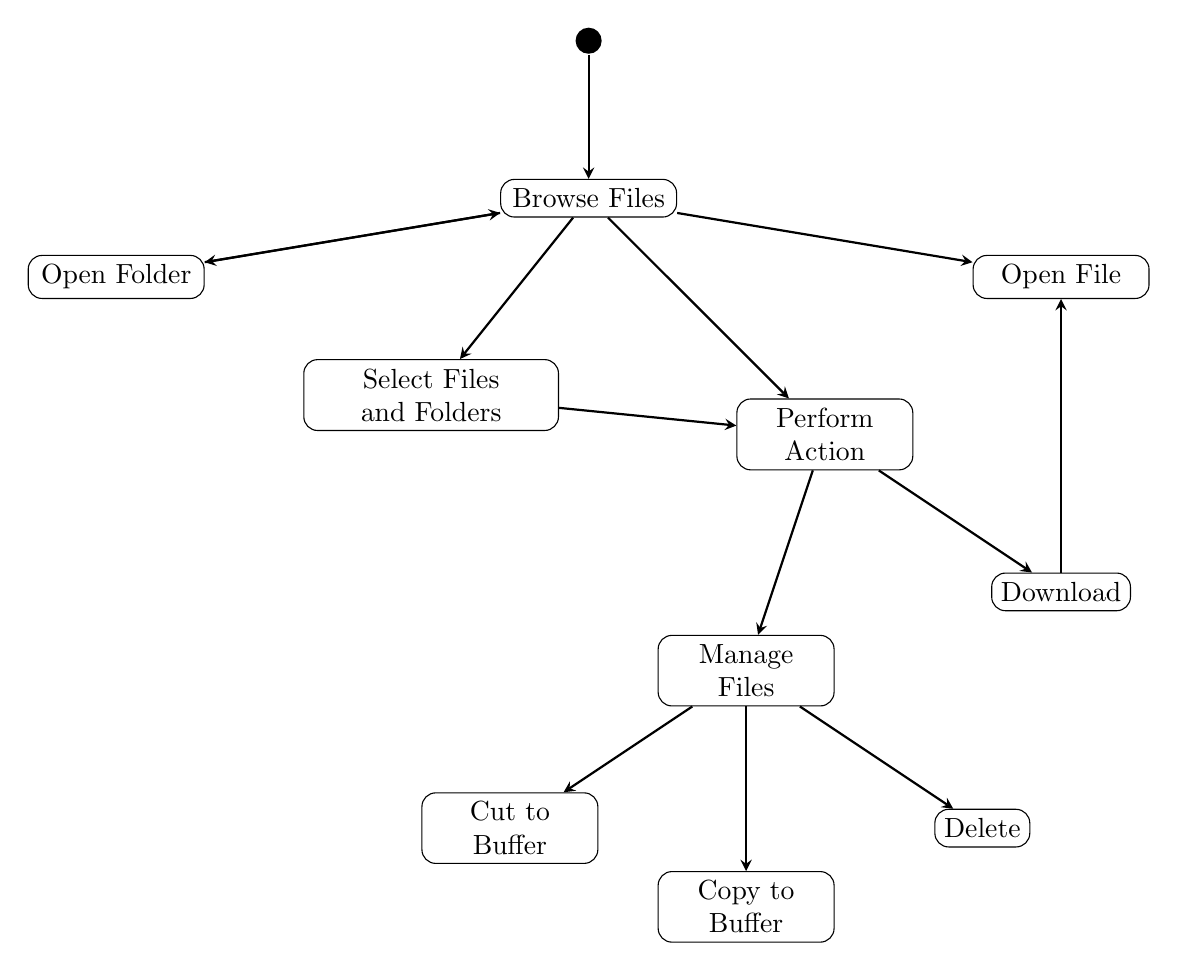
\begin{tikzpicture}[
		node distance=2cm,
		arrow/.style={thick,->,>=stealth},
		start/.style={fill=black,circle,thick},
		label/.style={rectangle, rounded corners=5, text centered, draw=black},
		fixlabel/.style={label, text width=2cm}
	]
	\node[start] at (0, 0) (start) {};
	\node[fixlabel] at (0, -2) (browse) {Browse Files};
	\node[fixlabel] at (-6, -3) (ofolder) {Open Folder};
	\node[fixlabel] at (6, -3) (ofile) {Open File};
	\node[label, text width=3cm] at (-2, -4.5) (select) {Select Files and Folders};
	\node[fixlabel] at (3, -5) (action) {Perform Action};
	\node[label] at (6, -7) (download) {Download};
	\node[fixlabel] at (2, -8) (manage) {Manage Files};
	\node[fixlabel] at (-1, -10) (cut) {Cut to Buffer};
	\node[fixlabel] at (2, -11) (copy) {Copy to Buffer};
	\node[label] at (5, -10) (delete) {Delete};

	\draw[arrow] (start) -- (browse);
	\draw[arrow] (browse) -- (ofile);
	\draw[arrow] (browse) -- (ofolder);
	\draw[arrow] (ofolder) -- (browse);
	\draw[arrow] (browse) -- (select);
	\draw[arrow] (browse) -- (action);
	\draw[arrow] (select) -- (action);
	\draw[arrow] (action) -- (manage);
	\draw[arrow] (action) -- (download);
	\draw[arrow] (download) -- (ofile);
	\draw[arrow] (manage) -- (cut);
	\draw[arrow] (manage) -- (copy);
	\draw[arrow] (manage) -- (delete);
\end{tikzpicture}
\end{center}
\vfill


\section{Database}
\vfill
\begin{center}
Representation of File Metadata in File System \\
\begin{tabular}{ | m{4cm} | m{3cm} | m{3cm} | m{3cm} | }
	\hline
	\thead{Attribute} &
	\thead{DataType} &
	\thead{Size} &
	\thead{Retrieval} \\
	\hline\hline
	Name               & Chars    & 255 Bytes & Primary Key \\
	Permissions        & Octal    & 4 Bytes   & Not Null \\
	User UID           & Integer  & 4 Bytes   & Not Null \\
	Group GID          & Integer  & 4 Bytes   & Not Null \\
	Modification Time  & Time     & 4 Bytes   & Not Null \\ \hline
\end{tabular}
\end{center}
\vfill


\section{Gantt Chart}
\vfill
\begin{center}
\begin{ganttchart}[
		hgrid=true,
		vgrid={*2{dotted}, {dashed}, *3{dotted}, {dashed}, *4{dotted}, {dashed}},
		y unit chart=0.8cm,
		title height=1,
		expand chart=\textwidth,
		bar label node/.append style={align=right},
		bar height=0.5,
		exed/.style={bar top shift=0.5},
		real/.style={bar top shift=0.1, bar/.append style={fill=black}},
	]{1}{15}
	\gantttitle{2024}{15} \ganttnewline[draw=none]
	\gantttitle{June}{3}
	\gantttitle{July}{4}
	\gantttitle{August}{5}
	\gantttitle{September}{3} \\
	\gantttitlelist{1,...,3}{1}
	\gantttitlelist{1,...,4}{1}
	\gantttitlelist{1,...,5}{1}
	\gantttitlelist{1,...,3}{1} \\
	\ganttbar[exed]{Requirements \\ Specification}{1}{1} \\
	\ganttbar[real]{}{1}{2} \\
	\ganttbar[exed]{Analysis}{2}{3} \\
	\ganttbar[real]{}{3}{4} \\
	\ganttbar[exed]{Design}{4}{5} \\
	\ganttbar[real]{}{5}{7} \\
	\ganttbar[exed]{Coding and \\ Testing}{6}{11} \\
	\ganttbar[real]{}{8}{12} \\
	\ganttbar[exed]{Implementation}{12}{13} \\
	\ganttbar[real]{}{13}{15} \\
\end{ganttchart}
\end{center}
\vfill


\end{document}

